% Options for packages loaded elsewhere
\PassOptionsToPackage{unicode}{hyperref}
\PassOptionsToPackage{hyphens}{url}
\documentclass[
  american,
  12pt,
  letterpaper,
]{article}
\usepackage{xcolor}
\usepackage{amsmath,amssymb}
\setcounter{secnumdepth}{5}
\usepackage{iftex}
\ifPDFTeX
  \usepackage[T1]{fontenc}
  \usepackage[utf8]{inputenc}
  \usepackage{textcomp} % provide euro and other symbols
\else % if luatex or xetex
  \usepackage{unicode-math} % this also loads fontspec
  \defaultfontfeatures{Scale=MatchLowercase}
  \defaultfontfeatures[\rmfamily]{Ligatures=TeX,Scale=1}
\fi
\usepackage{lmodern}
\ifPDFTeX\else
  % xetex/luatex font selection
\fi
% Use upquote if available, for straight quotes in verbatim environments
\IfFileExists{upquote.sty}{\usepackage{upquote}}{}
\IfFileExists{microtype.sty}{% use microtype if available
  \usepackage[]{microtype}
  \UseMicrotypeSet[protrusion]{basicmath} % disable protrusion for tt fonts
}{}
\makeatletter
\@ifundefined{KOMAClassName}{% if non-KOMA class
  \IfFileExists{parskip.sty}{%
    \usepackage{parskip}
  }{% else
    \setlength{\parindent}{0pt}
    \setlength{\parskip}{6pt plus 2pt minus 1pt}}
}{% if KOMA class
  \KOMAoptions{parskip=half}}
\makeatother
\usepackage{graphicx}
\makeatletter
\newsavebox\pandoc@box
\newcommand*\pandocbounded[1]{% scales image to fit in text height/width
  \sbox\pandoc@box{#1}%
  \Gscale@div\@tempa{\textheight}{\dimexpr\ht\pandoc@box+\dp\pandoc@box\relax}%
  \Gscale@div\@tempb{\linewidth}{\wd\pandoc@box}%
  \ifdim\@tempb\p@<\@tempa\p@\let\@tempa\@tempb\fi% select the smaller of both
  \ifdim\@tempa\p@<\p@\scalebox{\@tempa}{\usebox\pandoc@box}%
  \else\usebox{\pandoc@box}%
  \fi%
}
% Set default figure placement to htbp
\def\fps@figure{htbp}
\makeatother
\ifLuaTeX
\usepackage[bidi=basic,shorthands=off]{babel}
\else
\usepackage[bidi=default,shorthands=off]{babel}
\fi
\ifLuaTeX
  \usepackage{selnolig} % disable illegal ligatures
\fi
\setlength{\emergencystretch}{3em} % prevent overfull lines
\providecommand{\tightlist}{%
  \setlength{\itemsep}{0pt}\setlength{\parskip}{0pt}}
\usepackage[margin=1.24in]{geometry}
\usepackage{setspace}
\usepackage{graphicx}
\usepackage{xcolor}
\usepackage{helvet}
\usepackage{titlesec}
\usepackage{fancyhdr}
\usepackage{booktabs}
\usepackage{longtable}
\usepackage{array}
\usepackage{hyperref}
\definecolor{BookGold}{HTML}{FFD166}
\definecolor{BookBone}{HTML}{F6E8C8}
\definecolor{BookEmber}{HTML}{FF5E3A}
\definecolor{BookInk}{HTML}{12171F}
\renewcommand{\familydefault}{\rmdefault}
\setstretch{1.31}
\setlength{\parindent}{0pt}
\setlength{\parskip}{1.05em}
\raggedbottom
\titleformat{\section}{\normalfont\Large\bfseries\sffamily\color{BookEmber}}{\thesection}{0.7em}{}
\titleformat{\subsection}{\normalfont\large\bfseries\sffamily\color{BookGold}}{\thesubsection}{0.7em}{}
\hypersetup{
  colorlinks=true,
  linkcolor=BookEmber,
  urlcolor=BookEmber,
  citecolor=BookEmber
}
\pagestyle{fancy}
\fancyhf{}
\fancyhead[L]{\sffamily\small\textcolor{BookInk}{Children of the Feed}}
\fancyhead[R]{\sffamily\small\textcolor{BookInk}{\nouppercase{\leftmark}}}
\fancyfoot[C]{\sffamily\small\thepage}
\setlength{\headheight}{14pt}
\usepackage{bookmark}
\IfFileExists{xurl.sty}{\usepackage{xurl}}{} % add URL line breaks if available
\urlstyle{same}
% fallback for those not using the hyperref driver hyperxmp:
\makeatletter
\@ifundefined{xmpquote}{\newcommand{\xmpquote}[1]{#1}}{}
\makeatother
\hypersetup{
  pdftitle={The Layoff Ritual},
  pdflang={en-US},
  hidelinks,
  pdfcreator={LaTeX via pandoc}}

\title{The Layoff Ritual}
\author{}
\date{}

\begin{document}
\maketitle

\section{The Layoff Ritual}\label{the-layoff-ritual}

\subsection{Deck}\label{deck}

The machine did not only learn from workers. It was used to discipline
them.

\begin{figure}
\centering
\pandocbounded{
\includegraphics[keepaspectratio,alt={Chapter 05 cover}]{../assets/generated/covers/05_the-layoff-ritual_cover.png}}
\caption{Chapter 05 cover}
\end{figure}

\subsection{Opening}\label{opening}

The same industry that spent years treating elite technical workers like
golden blood suddenly found a very different vocabulary for them the
moment the market tightened.

Not builders.

Headcount.

Not talent.

Cost centers.

Not the future.

Excess.

Not family.

A line item.

If you worked in or around tech during that shift, you could feel the
betrayal almost before you could explain it. The vibes changed first.
Then the language changed. Then the org charts changed. Then people
disappeared.

One week it was founder talk, mission talk, future talk. The next week
it was nervous Slack threads, recruiter rumors, vague calendar holds,
and the weird quiet that hits an office when everybody already knows the
spreadsheet has started deciding who counts.

\subsection{Main Narrative}\label{main-narrative}

One of the cleanest lies of the AI era is that the layoffs were simple
proof that the machines had already made people obsolete. It is a neat
story, which is exactly why capital liked it. But the documentary record
is messier than that, and the mess is the point.

The correction was already forming.

Post-pandemic overhiring mattered.

Interest-rate pressure mattered.

Margin anxiety mattered.

Investor demands mattered.

Tax treatment changes such as Section 174 mattered.

The entire vibe shift from growth worship to efficiency worship
mattered.

AI did not create all of that from zero.

AI gave it a sacred language.

That language was wildly useful because it turned a financial and
strategic correction into a civilizational necessity. Once executives
could say ``we are reorganizing for the AI future,'' the cuts started
sounding visionary instead of extractive. Once a company could claim it
was flattening teams, driving efficiency, or reallocating toward
intelligence infrastructure, the human cost was wrapped in inevitability
language.

That is why the word ritual fits. A ritual is not just an event. It is
an event arranged to teach everyone something. The layoff wave taught
workers several lessons at once.

First: your talent is celebrated when growth needs your aura.

Second: your security evaporates when the macro story changes.

Third: a machine trained partly on the digital world you helped build
can be invoked rhetorically against you whether or not it has literally
replaced you in any clean technical sense.

That third lesson is one of the ugliest in the whole book. The same
ecosystem that harvested human labor, open knowledge, collective code,
and community-built expertise suddenly discovered the strategic value of
telling workers that their bargaining position had weakened because
intelligence itself was being automated. Sometimes there was a real
productivity shift underneath that claim. Often there was also narrative
theater doing a lot of heavy lifting.

The theater matters because it disciplines the surviving workforce even
when no full replacement has happened yet. If everyone around you is
being told that AI is the next productivity baseline, then the meaning
of your own labor changes even before your job does. You are expected to
output more, faster, with fewer people, while the company claims it is
simply adapting to the future.

That does something to worker psychology.

It narrows negotiation.

It weakens solidarity.

It makes resistance feel old-fashioned.

It makes management sound like history itself.

And because so many younger workers had been taught to treat tech not
just as employment but as identity, the hit landed deeper than a normal
recession story. The industry had sold a whole emotional package with
the paycheck: the mission, the campus, the perks, the myth that shipping
fast meant living at the frontier. Then the frontier started talking
back in cost-accounting language.

And because so much of the sector spent years mythologizing technical
labor as the engine of everything, the reversal hit with a particularly
disorienting force. Engineers were not only employees in this story.
They were social symbols. They were the proof that the future had
prestige, that software had winners, that intelligence still had upward
mobility attached to it. Then, when the correction arrived, the
symbolism snapped.

Suddenly the worker was not the future.

The worker was drag on margin.

That is not the whole story, of course. Some firms were genuinely
bloated. Some teams were real duplicates. Some pandemic-era hiring waves
were unsustainable in obvious ways. The point of this chapter is not to
romanticize every role or deny that labor markets swing. The point is to
stop accepting the flattering lie that the cuts can be fully explained
as purely technical progress.

They cannot.

Part of what made the story so effective was that it contained enough
truth to move fast. Yes, some automation tools were improving. Yes, some
companies had hired like zero-rate euphoria would last forever. Yes,
some orgs were padded. But that is exactly why the narrative worked: it
compressed multiple causes into one clean moral signal. The future
belongs to leaner firms and machine-assisted output, so anyone
questioning the cuts can be framed as arguing with reality itself.

The causal picture is layered:

financial correction,

tax treatment pressure,

capital-market discipline,

post-pandemic normalization,

efficiency language,

and then AI as legitimizing narrative layered on top.

That layered explanation is more uncomfortable than the simple one
because it reveals how power works in grown-up markets. The machine does
not need to fully replace the worker to lower the worker's leverage. It
only needs to become believable enough as a management story.

\begin{figure}
\centering
\pandocbounded{
\includegraphics[keepaspectratio,alt={Chapter 05 narrative illustration B}]{../assets/generated/illustrations/05_the-layoff-ritual_scene_b.png}}
\caption{Chapter 05 narrative illustration B}
\end{figure}

This is also where Section 174 matters in a way normal public discourse
almost never explains well. The rule change did not magically cause
every layoff by itself, and pretending it did would be sloppy. But it
did change how software and research spending hit the books, which
matters in a sector addicted to growth optics and investor signaling. If
labor once looked like expansion, parts of that same labor could
suddenly look like a cleaner thing to rationalize, defer, or cut. In
plain English: accounting pressure met macro pressure, then got narrated
through efficiency language that was unusually easy to fuse with AI
hype.

And when that fusion happened, workers were asked to internalize the
logic as common sense. Be grateful you are still here. Learn the tools
faster. Ship more with less. Treat the shrinking team as proof of
strategic maturity. Pretend the sprint did not just become a slow
emergency. A whole generation of technical workers got a brutal
education in how quickly ``the future'' turns on labor once capital
decides the valuation story needs a new costume.

\begin{figure}
\centering
\pandocbounded{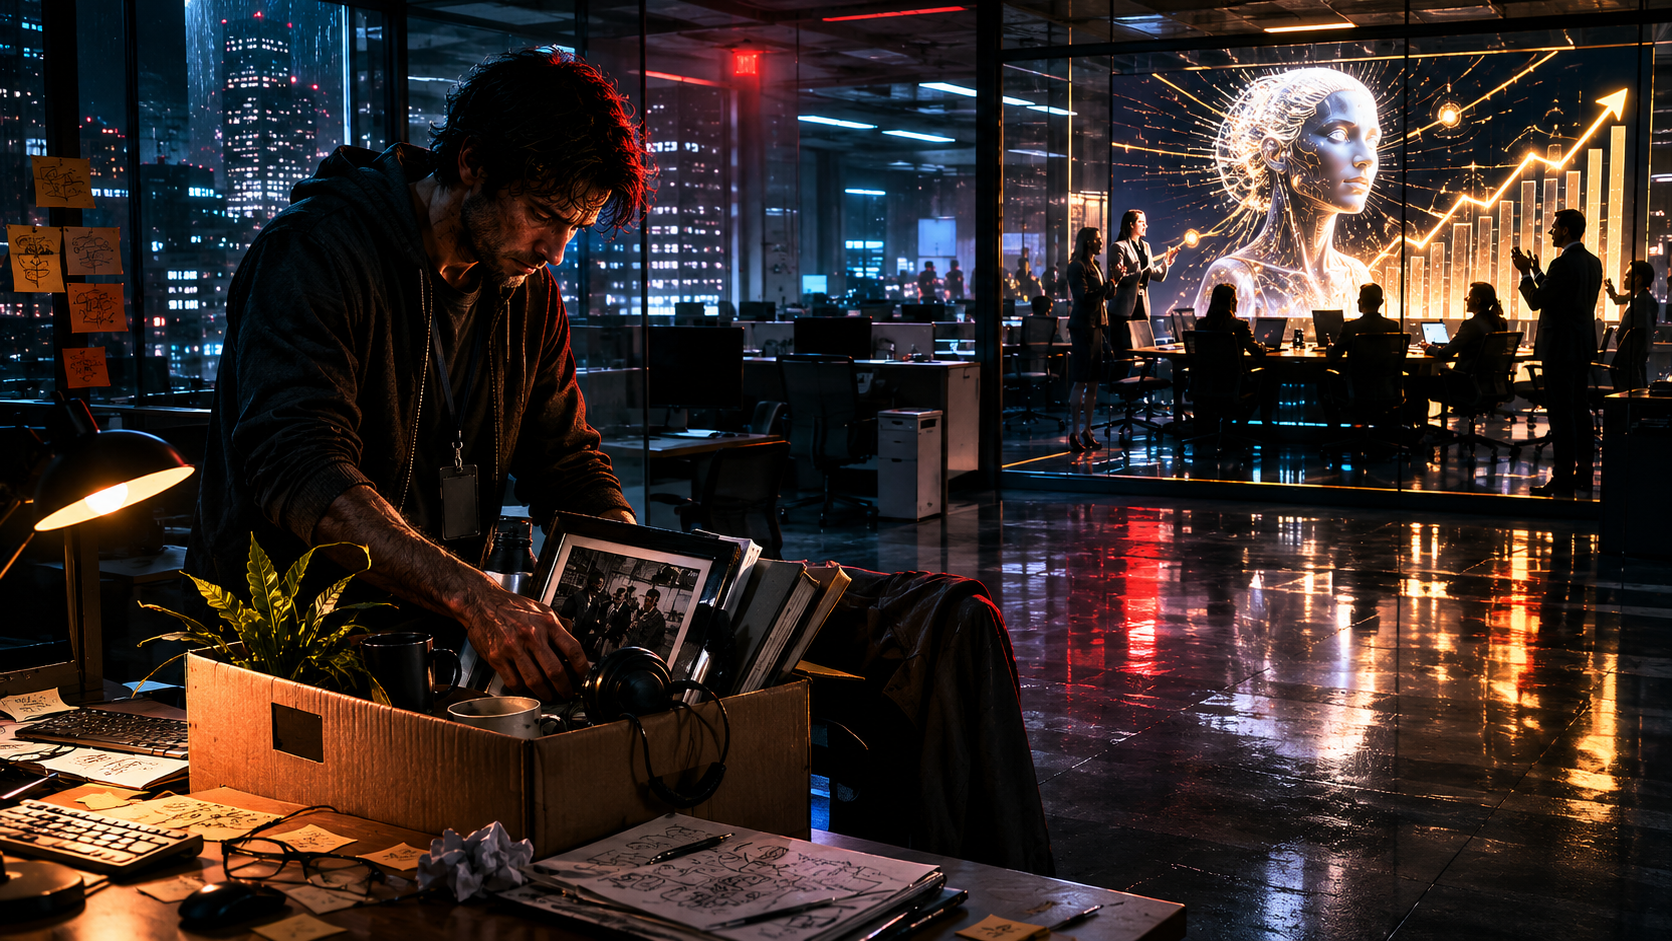
\includegraphics[keepaspectratio,alt={Chapter 05 narrative illustration}]{../assets/generated/illustrations/05_the-layoff-ritual_scene_a.png}}
\caption{Chapter 05 narrative illustration}
\end{figure}

That is the real weaponization of inevitability.

The machine becomes an alibi before it becomes a total substitute.

\begin{figure}
\centering
\pandocbounded{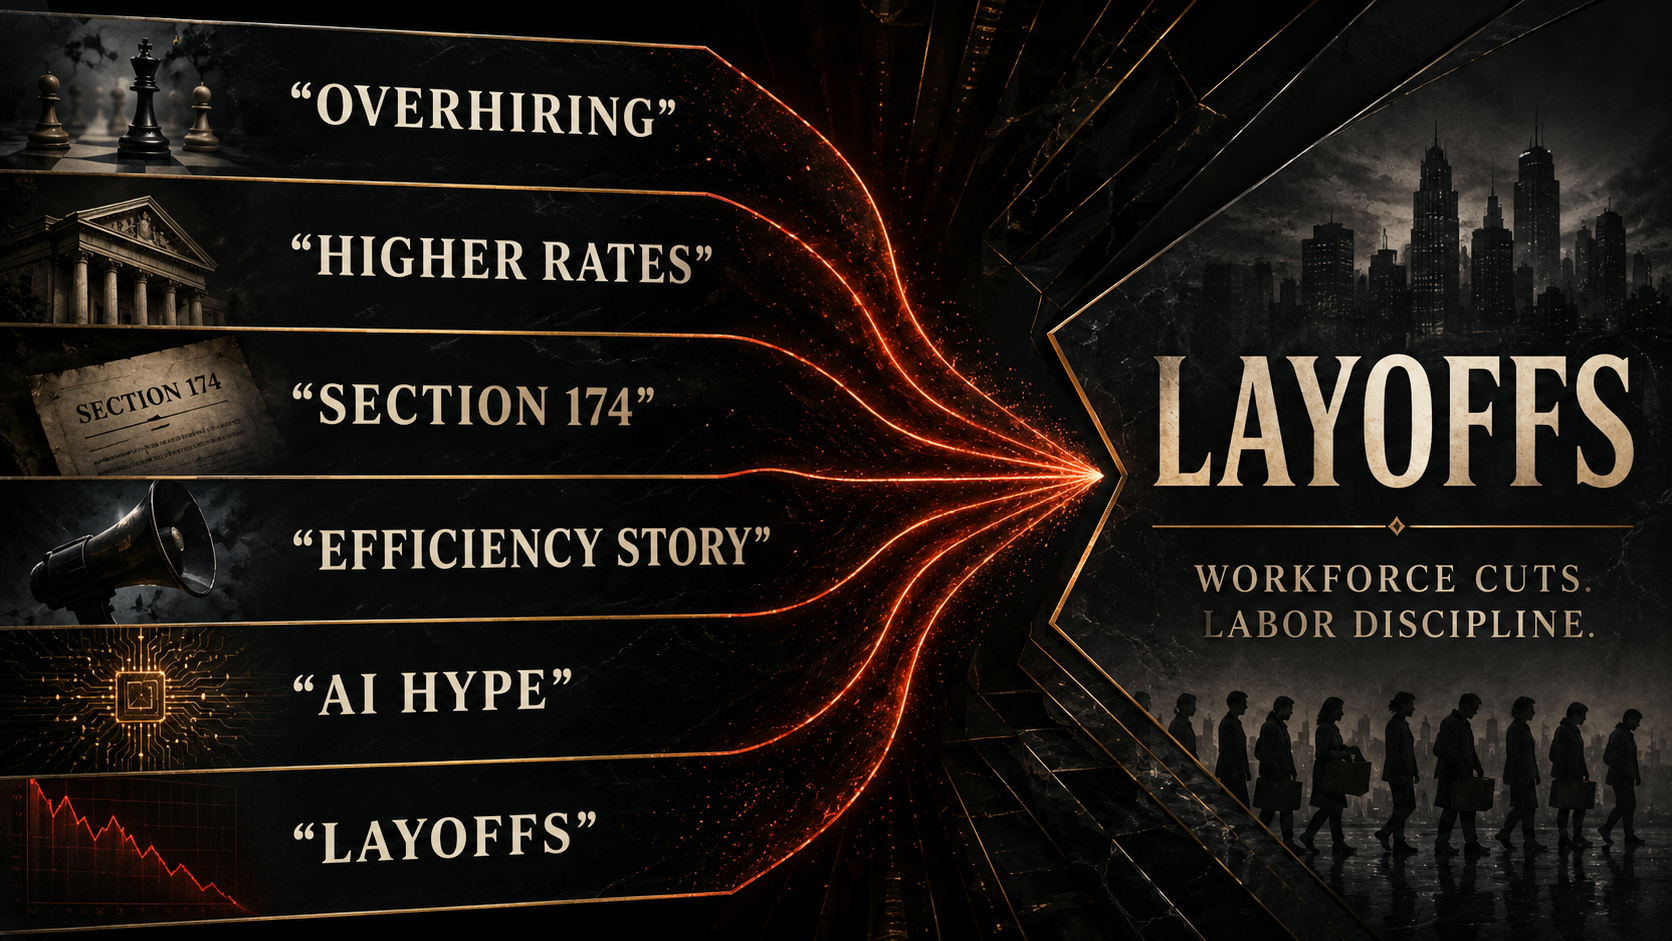
\includegraphics[keepaspectratio,alt={Chapter 05 infographic}]{../assets/generated/infographics/05_the-layoff-ritual_infographic_a.png}}
\caption{Chapter 05 infographic}
\end{figure}

And for middle-class technical workers, that alibi is politically
important because it shows how quickly a sector can move from talent
hoarding to labor disciplining once valuation logic changes. Companies
do not only hire because they need the exact current output. Sometimes
they hire to capture strategic labor, defend market position, signal
momentum, and build the story that justifies extraordinary valuation.
When that story changes, the same surplus labor that once inflated
prestige becomes the easiest thing to cut.

Workers experience the fall emotionally.

Finance experiences it narratively.

AI helped close that gap.

It let boards, executives, and markets say: this is not simply
retrenchment. This is modernization.

That word did serious ideological work. Modernization sounds clean.
Mature. Inevitable. Like no one made a choice and history just showed up
with a knife. But what many workers actually lived through felt less
like elegant modernization and more like class discipline in premium
branding: fewer people, more output, more pressure, more internal AI
mandates, more expectation that one person should now carry what used to
be one-and-a-half jobs.

That claim will keep showing up unless readers learn how to hear it
properly.

Modernization for whom?

Efficiency for whom?

Productivity against which denominator?

Innovation at whose cost?

When a firm that benefited from a decade of elite technical labor
suddenly starts talking like labor itself is a transitional
inconvenience, that is not just strategy. It is class reordering under
high-status language.

That matters because the future of AI is not only a story about
consumers and creators. It is also a story about the technical middle
class. The people who built systems, shipped products, made
infrastructure legible, staffed teams, documented knowledge, trained
juniors, and held together modern software organizations are being told
in real time that the very abstraction layer built from collective
digital life now justifies doing more with less.

The insult is historic.

But it is also clarifying.

\begin{figure}
\centering
\pandocbounded{
\includegraphics[keepaspectratio,alt={Chapter 05 narrative illustration C}]{../assets/generated/illustrations/05_the-layoff-ritual_scene_c.png}}
\caption{Chapter 05 narrative illustration C}
\end{figure}

It reveals where ownership sits.

It also reveals the labor logic of technofeudalism. The serf matters
until the lord finds a lower-friction way to extract the harvest. In the
digital version, elite labor is praised while it is scarce, strategic,
and valuation-friendly. Then, once enough code, enough process, enough
documentation, and enough machine leverage accumulate, the same labor is
told to accept weaker security in the name of progress. That is not a
glitch in the story. It is the story.

For readers outside tech, this chapter matters because the pattern does
not stay inside engineering orgs. It leaks outward into copywriting,
design, support, teaching, analysis, journalism, legal prep,
translation, and all the middle layers of knowledge work. The prestige
version shows up first in software because software had the capital and
the mythology. The discipline mechanism spreads later. What gets tested
on engineers today gets marketed to everyone else tomorrow as the
responsible way to live with AI.

\subsection{Research Basis}\label{research-basis}

This chapter adapts the documentary argument developed in the research
paper
\href{../../papers/html/05_talent-overhiring-layoffs_paper.html}{\textbf{Chapter
05: Talent, Overhiring, Valuation, and Layoffs}}. The PDF version is
\href{../../papers/pdf/05_talent-overhiring-layoffs_paper/05_talent-overhiring-layoffs_paper.pdf}{here}.
That paper ties labor correction to financial structure, Section 174,
post-pandemic excess, company efficiency language, and the strategic use
of AI rhetoric.

\subsection{Next}\label{next}

Once AI becomes a labor-disciplining story, it can also be sold in two
voices at once: dangerous enough to change history, friendly enough to
place in every workflow. The next chapter follows that contradiction.

\end{document}
